% --------------------------------------------------------------------
\documentclass{standalone}

\usepackage{mathtools}

\usepackage{tikz}
%\input{diagrammatics.tex}

\usetikzlibrary{decorations.markings}
\usetikzlibrary{arrows}
\usetikzlibrary{arrows.meta}
\usetikzlibrary{shapes.geometric}

\begin{document}
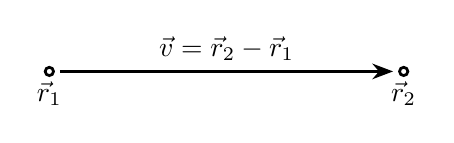
\begin{tikzpicture}[baseline, line width=1pt, scale=0.75]

  \begin{scope}[xshift=0.0cm, yshift=0.0cm]

  \draw (0,0) node [name=r1] {};
  \draw (6,0) node[name=r2] {};
  \draw [-Stealth] (r1) -- node[midway, above] {$\vec{v} = \vec{r}_2 - \vec{r}_1$} (r2);

  \draw (r1) circle [radius=2pt, fill=black!40];
  \draw (r2) circle [radius=2pt, fill=black!40];
  
  \draw (r1) node[below] {$\vec{r}_1$};
  \draw (r2) node[below] {$\vec{r}_2$};

  \end{scope}

\end{tikzpicture}
\end{document}
